\documentclass[a4paper, 16pt]{article}

\usepackage[czech]{babel}
\usepackage[utf8]{inputenc}
\usepackage[left=2cm, top=3cm, text={17cm, 24cm}]{geometry}
\usepackage{pdflscape}
\usepackage{graphicx}
\usepackage{picture}
\usepackage[dvipsnames]{xcolor}
\usepackage{float}


\begin{document}
    			\begin{center}
				{\LARGE
					Ukládání a příprava dat -- Projekt \\
					{\Large
					    Výsledky získané v rámci riešenia úloh \\[5mm]
					}
				}
				{\large
					Matej Berezný, Ondrej Valo, Švenk Adam \\	{\small xberez03, xvaloo00, xsvenk00}
					
				}
			\end{center}
			\vspace{0.7cm}

\section{1. dotaz skupiny A}

V rámci prvej úlohy bolo treba vygenerovať graf zobrazujúci vývoj covidovej situácie po mesiacoch. V grafe sú zobrazené hodnoty: počet novo nakazených za mesiac(\textcolor{orange}{oranžová}), počet novo vyliečených za mesiac(\textcolor{green}{zelená}), počet novo hospitalizovaných osôb za mesiac(\textcolor{blue}{modrá}) a počet vykonaných testov za mesiac(\textcolor{red}{červená}).
\begin{figure}[H] \centering
    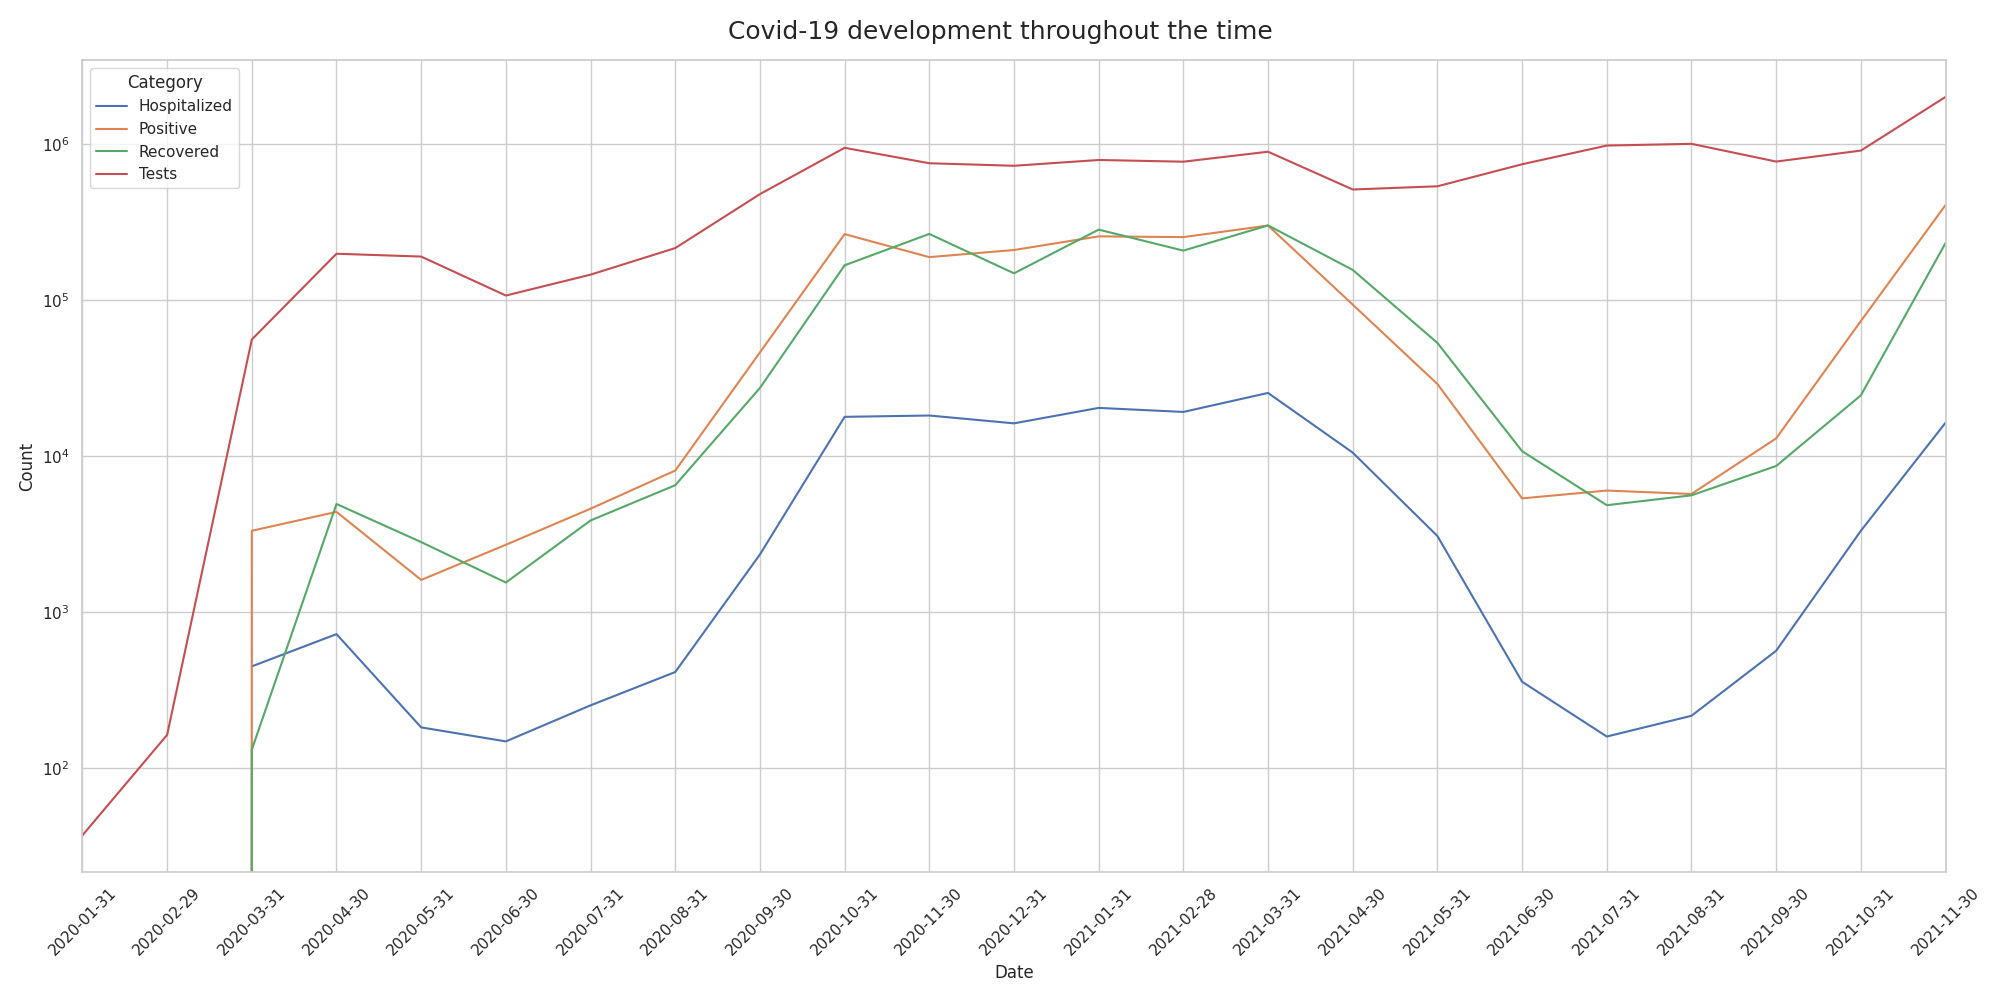
\includegraphics[width=\linewidth,height=5in]{Q1.png}
    \caption{Vývoj Covid-19 v priebehu času.}
    \label{graf_1}
\end{figure}

\newpage
\section{2. dotaz skupiny A}

V rámci druhej úlohy bolo treba vytvoriť krabicové grafy zobrazujúce rozloženie veku nakazených osôb v jednotlivých krajoch. Na grafe sú kraje zľava: Hlavné mesto Praha, Ústecký kraj, Zlínský kraj, Královéhradecký kraj, Středočeský kraj, Olomoucký kraj, Plzeňský kraj, Karlovarský kraj, Kraj Vysočina, Pardubický kraj, Jihomoravský kraj, Liberecký kraj, Moravskoslezský kraj, Jihočeský kraj.
\begin{figure}[H] \centering
    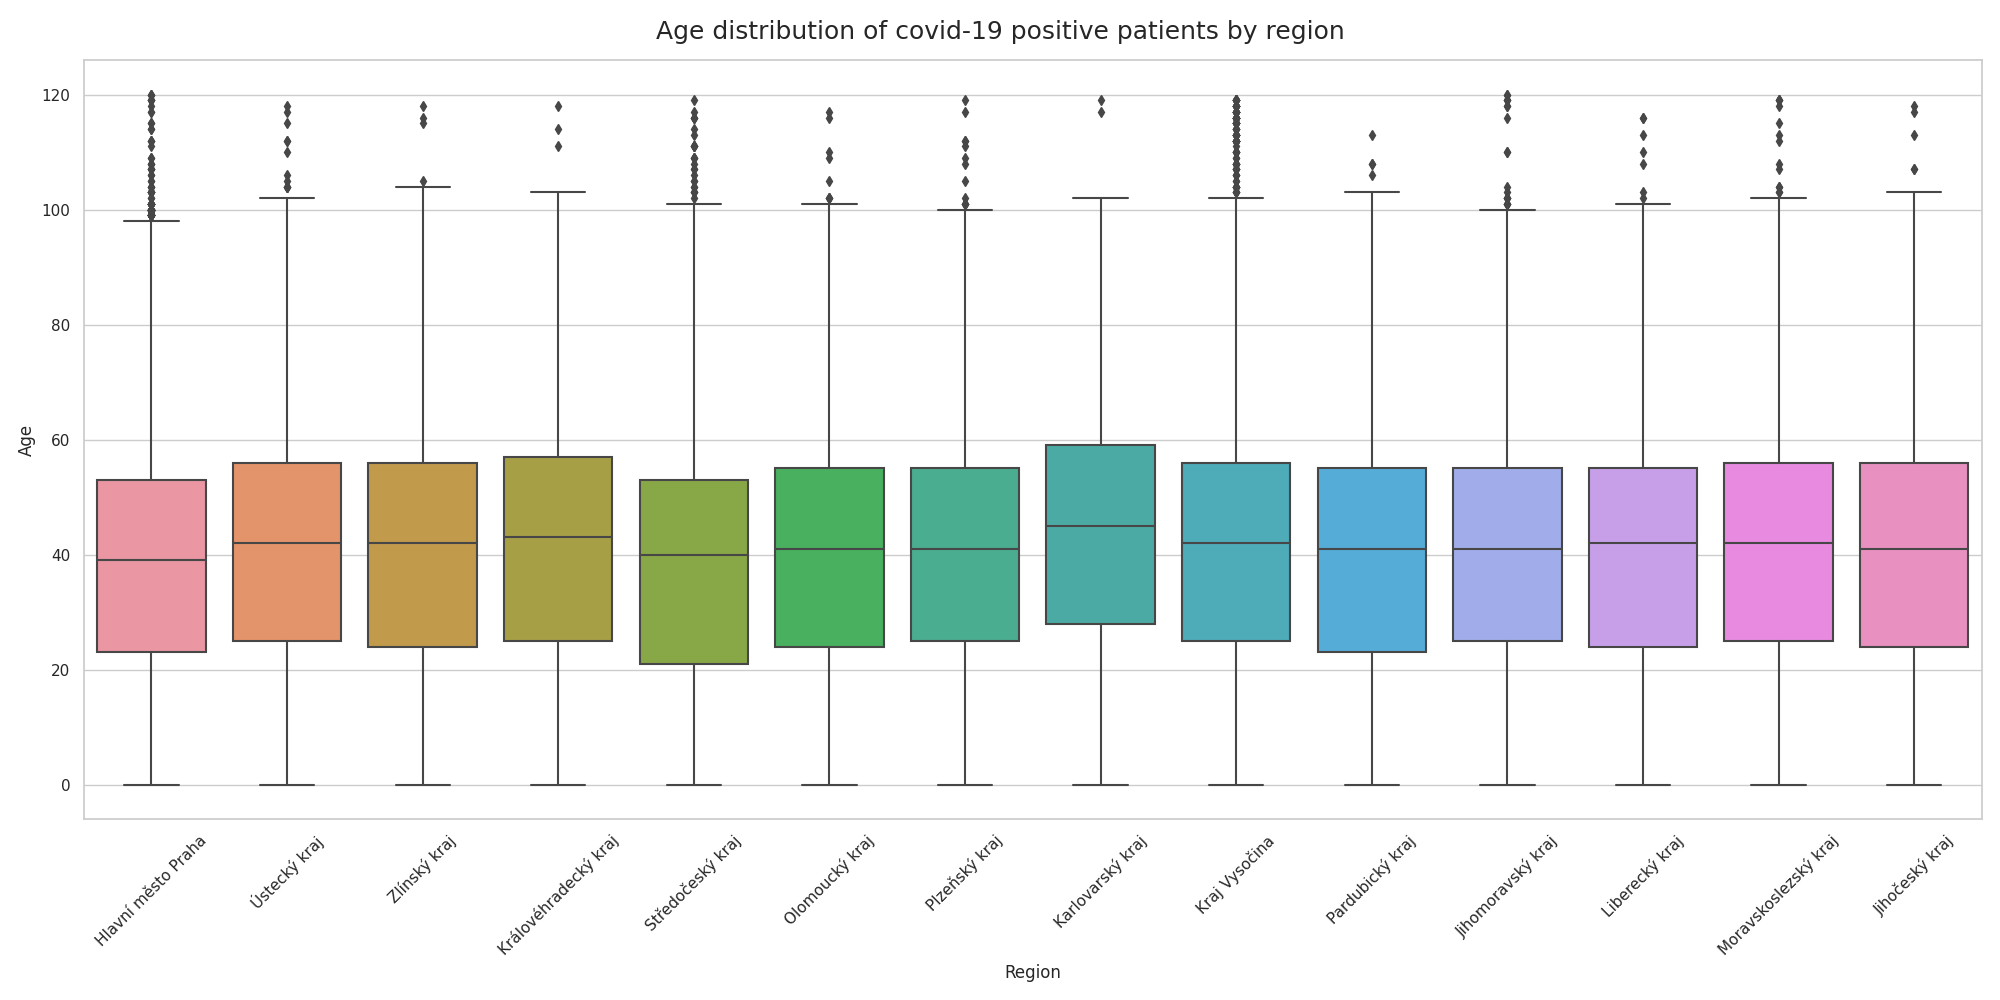
\includegraphics[width=\linewidth,height=5in]{Q2.png}
    \caption{Vekové rozloženie pacientov pozitívnych na covid-19 podľa regiónu.}
    \label{graf_2}
\end{figure}

\newpage
\section{Dotaz skupiny B}

V úlohe skupiny B bolo treba zostaviť 4 rebríčky krajov "best in covid" za posledné 4 štvrťroky. Ako kritérium bol braný počet novo nakazených prepočítaný na jedného obyvateľa kraja. A pre jeden štvrť rok vygenerovať graf, ktorý zobrazuje počet novo nakazených(\textcolor{BlueViolet}{tmavo modrá}), celkový počet obyvateľov(\textcolor{CornflowerBlue}{svetlo modrá}) a počet nakazených na jedného obyvateľa(\textcolor{red}{červená}). Počet nakazených na jedného obyvateľa bol vypočítaný ako \textit{počet nakazených v kraji/celková populácia v kraji} Graf \ref{graf_3} bol vygenerovaný na základe tabuľky \ref{table_1}

\begin{figure}[H] \centering
    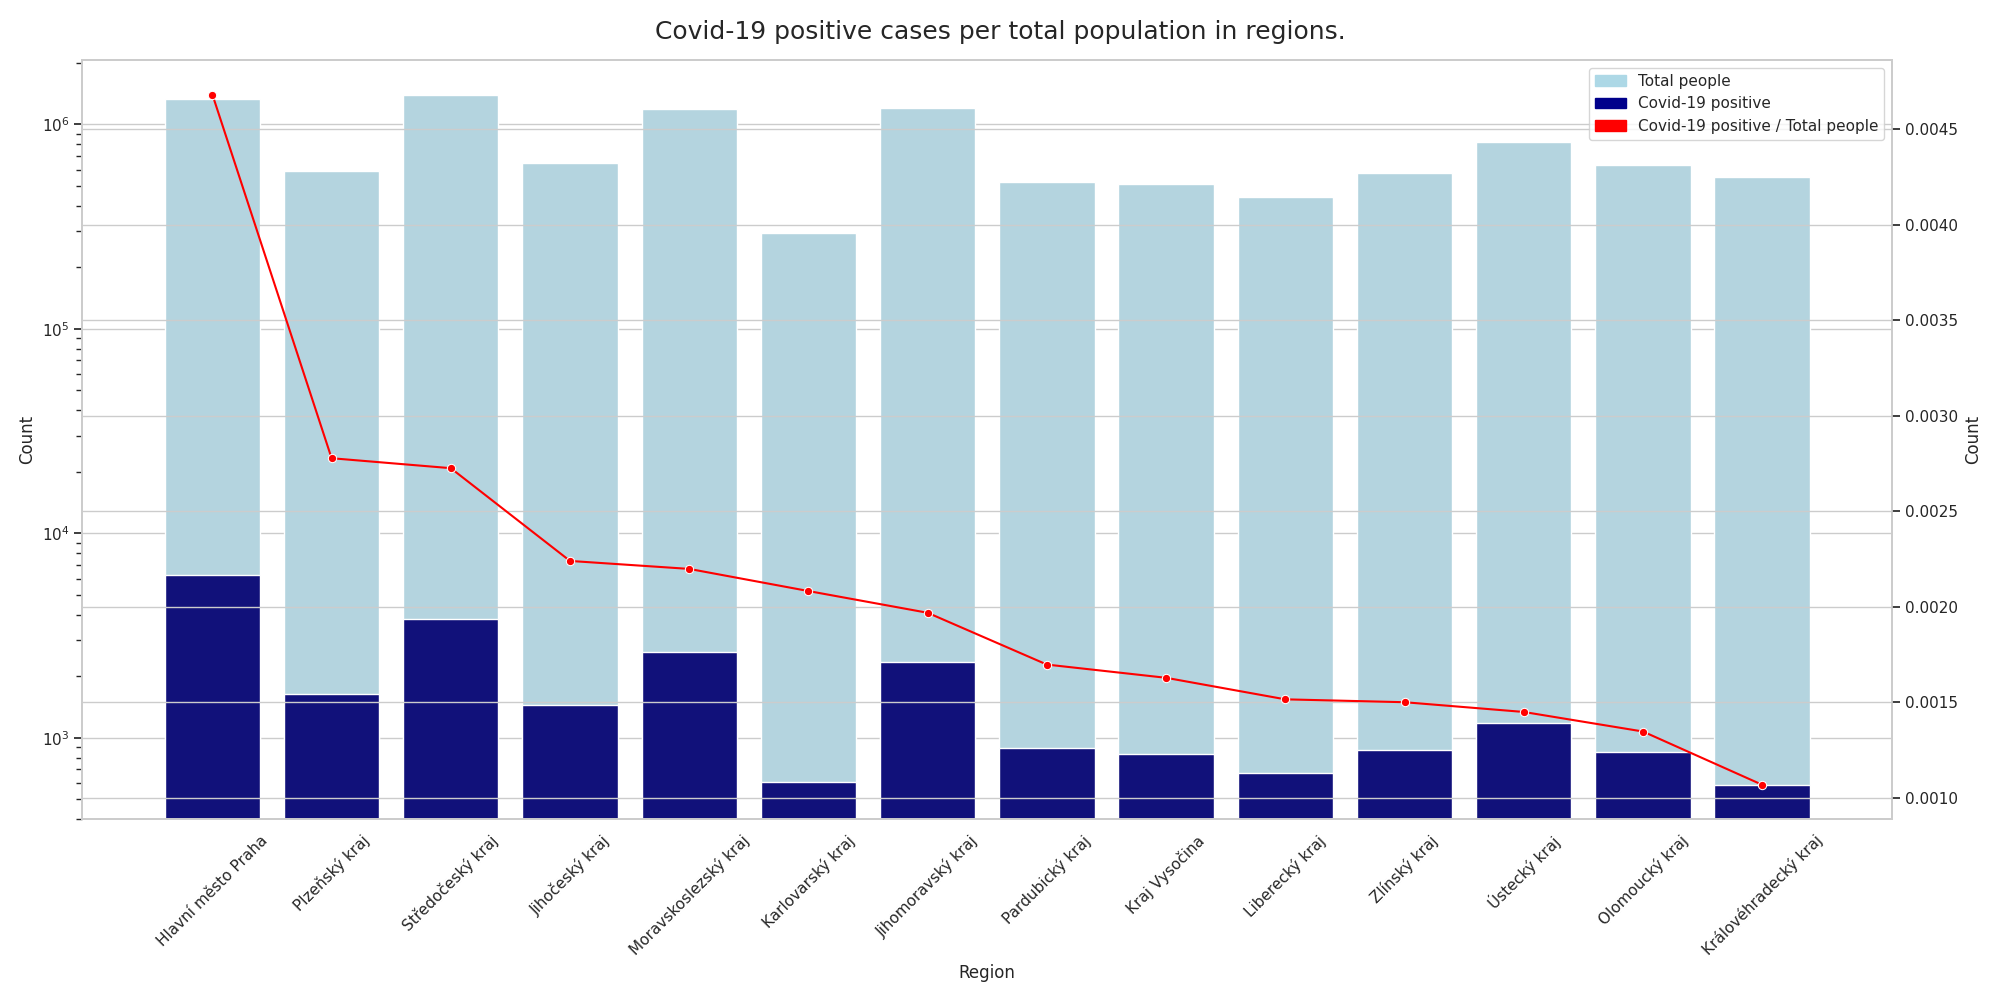
\includegraphics[width=\linewidth,height=3.5in]{QB.png}
    \caption{Pozitívne prípady Covid-19 na celkovú populáciu v regiónoch.}
    \label{graf_3}
\end{figure}

\begin{figure}[H] \centering
    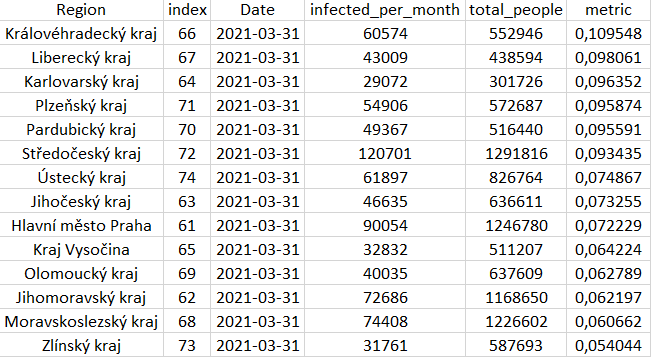
\includegraphics[width=\linewidth,height=3.5in]{B_0.png}
    \caption{Dáta Pozitívnych prípadov Covid-19 na celkovú populáciu v regiónoch za prvý štvrť rok.}
    \label{table_0}
\end{figure}

\begin{figure}[H] \centering
    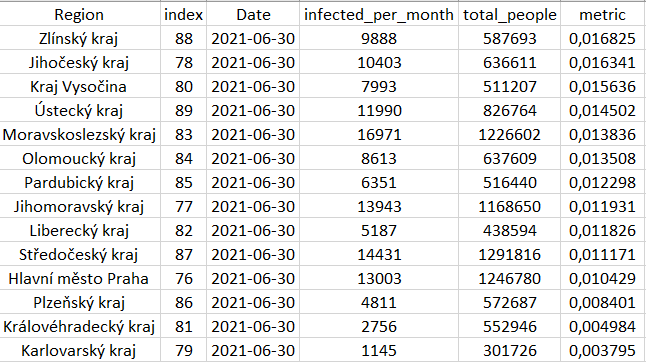
\includegraphics[width=\linewidth,height=3.5in]{B_1.png}
    \caption{Dáta Pozitívnych prípadov Covid-19 na celkovú populáciu v regiónoch za druhý štvrť rok.}
    \label{table_1}
\end{figure}

\begin{figure}[H] \centering
    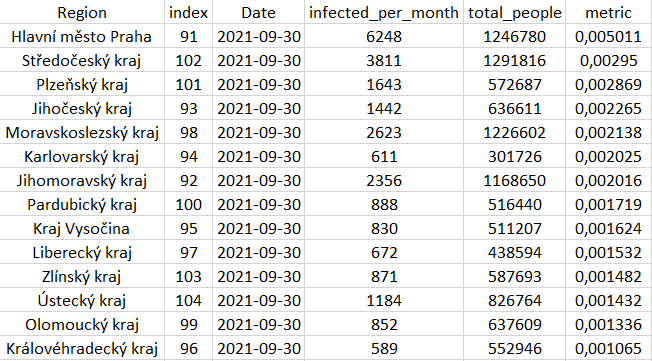
\includegraphics[width=\linewidth,height=3.5in]{B_2.png}
    \caption{Dáta Pozitívnych prípadov Covid-19 na celkovú populáciu v regiónoch za tretí štvrť rok.}
    \label{table_2}
\end{figure}

\begin{figure}[H] \centering
    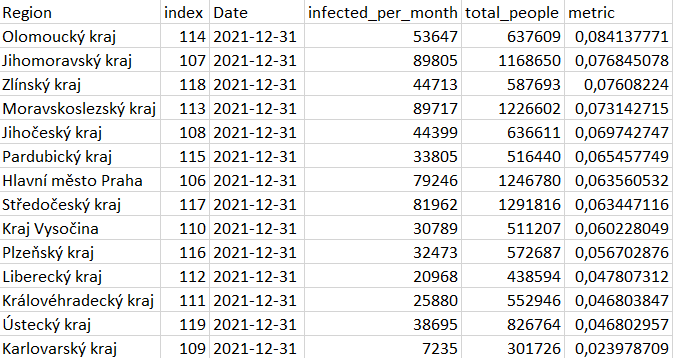
\includegraphics[width=\linewidth,height=3.5in]{B_3.png}
    \caption{Dáta Pozitívnych prípadov Covid-19 na celkovú populáciu v regiónoch za štvrtý štvrť rok.}
    \label{table_3}
\end{figure}



\section{Vlastný dotaz 1}

Prvý dotaz zobrazuje pomer medzi očkovanými (\textcolor{BlueViolet}{tmavo modré stĺpčeky}) a neočkovanými osobami(\textcolor{CornflowerBlue}{svetlo modré stĺpčeky}) z hľadiska počtu úmrtí (druhý stĺpec), počtu pacientov na JIP (prvý stĺpec), počtu hospitalizovaných pacientov (tretí stĺpec) a ich vzťahu k celkovej zaočkovanosti populácie (červená čiara) počas jednotlivých mesiacov. Pomer aj celková zaočkovanosť je vyjadrená v percentách z dôvodu veľkých rozdielov dát pre jednotlivé mesiace.

\begin{figure}[H] \centering
    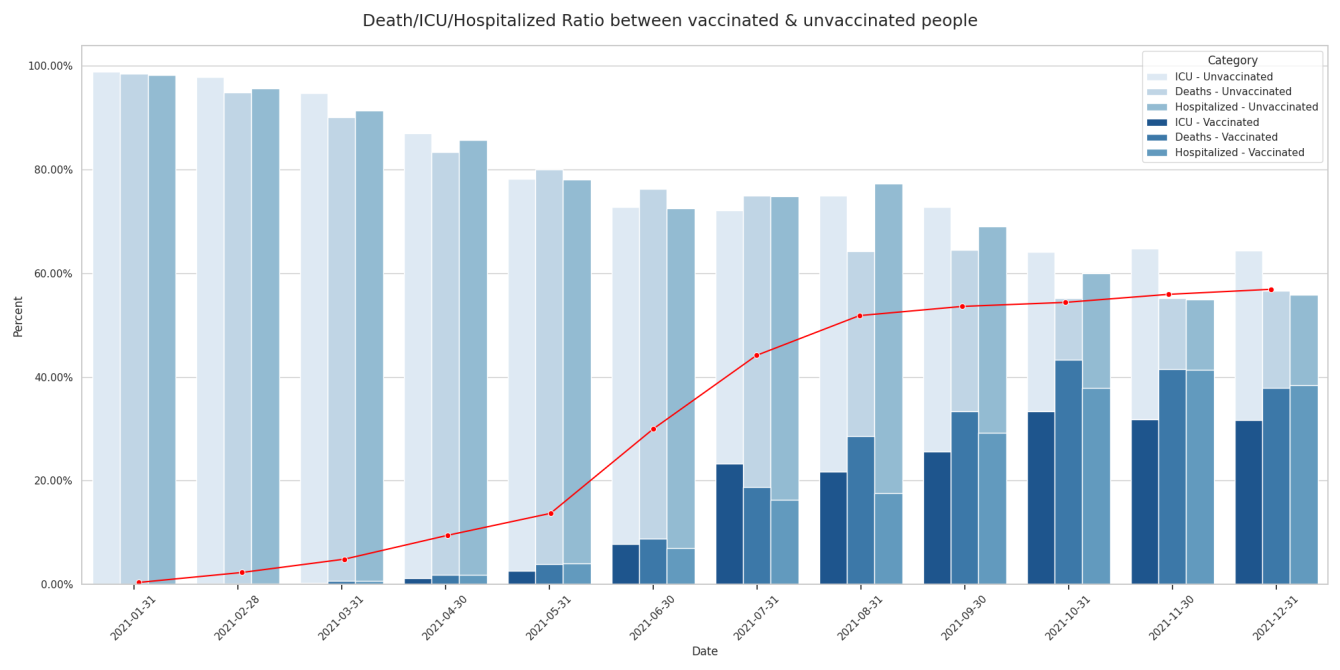
\includegraphics[width=\linewidth,height=3.5in]{QC1.png}
    \caption{Pomer úmrtí, JIP a hospitalizácie medzi očkovanými a neočkovanými osobami.}
    \label{graf_4}
\end{figure}

\section{Vlastný dotaz 2}

Druhý dotaz zobrazuje vývoj počtu pacientov s veľmi ťažkým priebehom ochorenia nachádajúcich sa na špeciálnych prístrojoch/oddeleniach (JIP, pľúcna ventilácia etc.) ku celkovému počtu nových prípadov ochorenia Covid-19 (hnedá farba) počas jednotlivých mesiacov.
\begin{figure}[H] \centering
    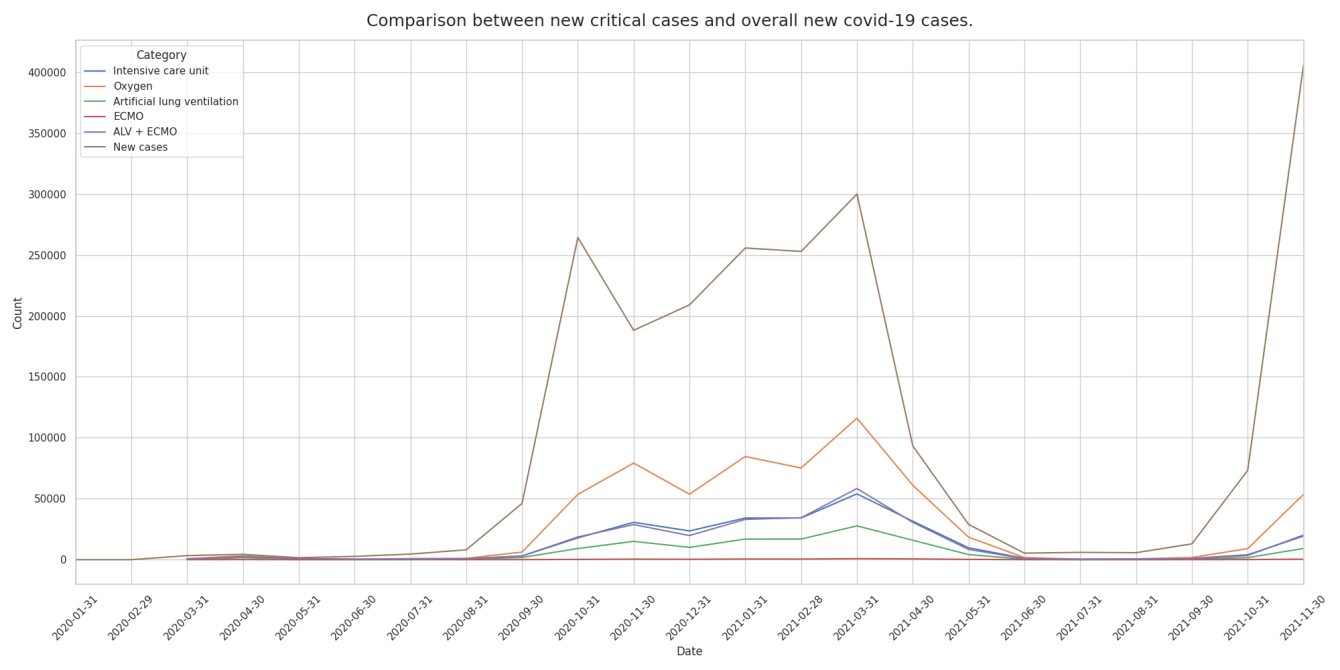
\includegraphics[width=\linewidth,height=3.5in]{QC2.png}
    \caption{Porovnanie medzi novými kritickými prípadmi a celkovo novými prípadmi COVID-19.}
    \label{graf_5}
\end{figure}

\newpage
\section{Dotaz skupiny C}

Cieľom úlohy skupiny C bolo vytvorenie súboru vo formáte CSV, ktorý bude možné predať dolovaciemu algoritmu. Predmetom dolovacieho algoritmu je vyhľadávanie miest (okresov), v ktorých je vývoj aktuálnej situácie týkajúcej sa šírenia ochorenia Covid-19 podobný. Normalizácia prebiehala výpočtom percentuálneho podielu počtu očkovanej populácie za obdobie posledných 4 štvrťrokov (čiže období posledného roka) vzhľadom na celkovú populáciu danej regionálnej oblasti. Diskretizáciu dát vychádza z kategórizácie percentuálneho počtu zaočkovanej populácie. Okrem dodaného súboru CSV, na ktorom je vykonaná normalizácia a diskretizácia, je dodávaný aj súbor vo formáte CSV bez týchto vykonaných úkonov. Zadanie vyžadovalo detekciu a nahradenie odľahlých hodnôt. Vzhľadom na vybratú tému a použité dátové kolekcie však nebolo možné detekovať a nahradiť odľahlé hodnoty, nakoľko takéto vykonanie nie je prospešné v prípade zvolenej témy. Výsledný súbor vo formáte CSV (konkrétne jeho časť) je možné vidieť na obrázku \ref{graf_c}).

\begin{figure}[H] \centering
    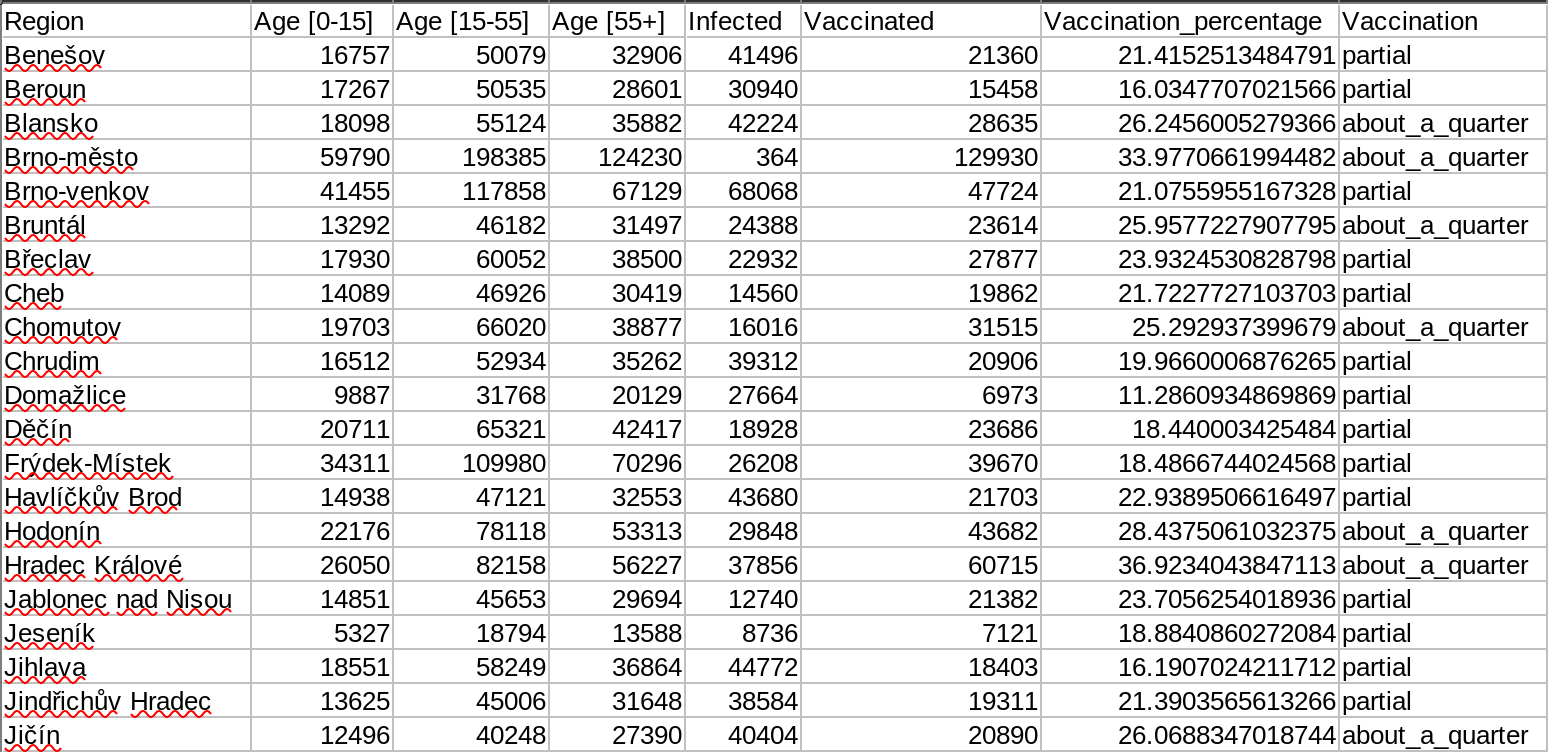
\includegraphics[width=\linewidth,height=3.5in]{queryC.png}
    \caption{Pripravené dáta pre dolovací algoritmus}
    \label{graf_c}
\end{figure}

	
\end{document}
